% Options for packages loaded elsewhere
\PassOptionsToPackage{unicode}{hyperref}
\PassOptionsToPackage{hyphens}{url}
%
\documentclass[
  english,
  man]{apa6}
\title{EDLD 640 Capstone}
\author{Diana DeWald\textsuperscript{1} \& Dare Baldwin\textsuperscript{1}}
\date{}

\usepackage{amsmath,amssymb}
\usepackage{lmodern}
\usepackage{iftex}
\ifPDFTeX
  \usepackage[T1]{fontenc}
  \usepackage[utf8]{inputenc}
  \usepackage{textcomp} % provide euro and other symbols
\else % if luatex or xetex
  \usepackage{unicode-math}
  \defaultfontfeatures{Scale=MatchLowercase}
  \defaultfontfeatures[\rmfamily]{Ligatures=TeX,Scale=1}
\fi
% Use upquote if available, for straight quotes in verbatim environments
\IfFileExists{upquote.sty}{\usepackage{upquote}}{}
\IfFileExists{microtype.sty}{% use microtype if available
  \usepackage[]{microtype}
  \UseMicrotypeSet[protrusion]{basicmath} % disable protrusion for tt fonts
}{}
\makeatletter
\@ifundefined{KOMAClassName}{% if non-KOMA class
  \IfFileExists{parskip.sty}{%
    \usepackage{parskip}
  }{% else
    \setlength{\parindent}{0pt}
    \setlength{\parskip}{6pt plus 2pt minus 1pt}}
}{% if KOMA class
  \KOMAoptions{parskip=half}}
\makeatother
\usepackage{xcolor}
\IfFileExists{xurl.sty}{\usepackage{xurl}}{} % add URL line breaks if available
\IfFileExists{bookmark.sty}{\usepackage{bookmark}}{\usepackage{hyperref}}
\hypersetup{
  pdftitle={EDLD 640 Capstone},
  pdfauthor={Diana DeWald1 \& Dare Baldwin1},
  pdflang={en-EN},
  pdfkeywords={causal learning models, pedagogy, text analysis},
  hidelinks,
  pdfcreator={LaTeX via pandoc}}
\urlstyle{same} % disable monospaced font for URLs
\usepackage{graphicx}
\makeatletter
\def\maxwidth{\ifdim\Gin@nat@width>\linewidth\linewidth\else\Gin@nat@width\fi}
\def\maxheight{\ifdim\Gin@nat@height>\textheight\textheight\else\Gin@nat@height\fi}
\makeatother
% Scale images if necessary, so that they will not overflow the page
% margins by default, and it is still possible to overwrite the defaults
% using explicit options in \includegraphics[width, height, ...]{}
\setkeys{Gin}{width=\maxwidth,height=\maxheight,keepaspectratio}
% Set default figure placement to htbp
\makeatletter
\def\fps@figure{htbp}
\makeatother
\setlength{\emergencystretch}{3em} % prevent overfull lines
\providecommand{\tightlist}{%
  \setlength{\itemsep}{0pt}\setlength{\parskip}{0pt}}
\setcounter{secnumdepth}{-\maxdimen} % remove section numbering
% Make \paragraph and \subparagraph free-standing
\ifx\paragraph\undefined\else
  \let\oldparagraph\paragraph
  \renewcommand{\paragraph}[1]{\oldparagraph{#1}\mbox{}}
\fi
\ifx\subparagraph\undefined\else
  \let\oldsubparagraph\subparagraph
  \renewcommand{\subparagraph}[1]{\oldsubparagraph{#1}\mbox{}}
\fi
\newlength{\cslhangindent}
\setlength{\cslhangindent}{1.5em}
\newlength{\csllabelwidth}
\setlength{\csllabelwidth}{3em}
\newlength{\cslentryspacingunit} % times entry-spacing
\setlength{\cslentryspacingunit}{\parskip}
\newenvironment{CSLReferences}[2] % #1 hanging-ident, #2 entry spacing
 {% don't indent paragraphs
  \setlength{\parindent}{0pt}
  % turn on hanging indent if param 1 is 1
  \ifodd #1
  \let\oldpar\par
  \def\par{\hangindent=\cslhangindent\oldpar}
  \fi
  % set entry spacing
  \setlength{\parskip}{#2\cslentryspacingunit}
 }%
 {}
\usepackage{calc}
\newcommand{\CSLBlock}[1]{#1\hfill\break}
\newcommand{\CSLLeftMargin}[1]{\parbox[t]{\csllabelwidth}{#1}}
\newcommand{\CSLRightInline}[1]{\parbox[t]{\linewidth - \csllabelwidth}{#1}\break}
\newcommand{\CSLIndent}[1]{\hspace{\cslhangindent}#1}
% Manuscript styling
\usepackage{upgreek}
\captionsetup{font=singlespacing,justification=justified}

% Table formatting
\usepackage{longtable}
\usepackage{lscape}
% \usepackage[counterclockwise]{rotating}   % Landscape page setup for large tables
\usepackage{multirow}		% Table styling
\usepackage{tabularx}		% Control Column width
\usepackage[flushleft]{threeparttable}	% Allows for three part tables with a specified notes section
\usepackage{threeparttablex}            % Lets threeparttable work with longtable

% Create new environments so endfloat can handle them
% \newenvironment{ltable}
%   {\begin{landscape}\centering\begin{threeparttable}}
%   {\end{threeparttable}\end{landscape}}
\newenvironment{lltable}{\begin{landscape}\centering\begin{ThreePartTable}}{\end{ThreePartTable}\end{landscape}}

% Enables adjusting longtable caption width to table width
% Solution found at http://golatex.de/longtable-mit-caption-so-breit-wie-die-tabelle-t15767.html
\makeatletter
\newcommand\LastLTentrywidth{1em}
\newlength\longtablewidth
\setlength{\longtablewidth}{1in}
\newcommand{\getlongtablewidth}{\begingroup \ifcsname LT@\roman{LT@tables}\endcsname \global\longtablewidth=0pt \renewcommand{\LT@entry}[2]{\global\advance\longtablewidth by ##2\relax\gdef\LastLTentrywidth{##2}}\@nameuse{LT@\roman{LT@tables}} \fi \endgroup}

% \setlength{\parindent}{0.5in}
% \setlength{\parskip}{0pt plus 0pt minus 0pt}

% \usepackage{etoolbox}
\makeatletter
\patchcmd{\HyOrg@maketitle}
  {\section{\normalfont\normalsize\abstractname}}
  {\section*{\normalfont\normalsize\abstractname}}
  {}{\typeout{Failed to patch abstract.}}
\patchcmd{\HyOrg@maketitle}
  {\section{\protect\normalfont{\@title}}}
  {\section*{\protect\normalfont{\@title}}}
  {}{\typeout{Failed to patch title.}}
\makeatother
\shorttitle{Natural Language Processing for Pedagogy}
\keywords{causal learning models, pedagogy, text analysis\newline\indent Word count: 944}
\DeclareDelayedFloatFlavor{ThreePartTable}{table}
\DeclareDelayedFloatFlavor{lltable}{table}
\DeclareDelayedFloatFlavor*{longtable}{table}
\makeatletter
\renewcommand{\efloat@iwrite}[1]{\immediate\expandafter\protected@write\csname efloat@post#1\endcsname{}}
\makeatother
\usepackage{lineno}

\linenumbers
\usepackage{csquotes}
\ifXeTeX
  % Load polyglossia as late as possible: uses bidi with RTL langages (e.g. Hebrew, Arabic)
  \usepackage{polyglossia}
  \setmainlanguage[]{english}
\else
  \usepackage[main=english]{babel}
% get rid of language-specific shorthands (see #6817):
\let\LanguageShortHands\languageshorthands
\def\languageshorthands#1{}
\fi
\ifLuaTeX
  \usepackage{selnolig}  % disable illegal ligatures
\fi


\affiliation{\vspace{0.5cm}\textsuperscript{1} University of Oregon}

\abstract{
(will change wording to past tense once project is completed, and will add in results and discussion summary)..

How is young children's exploration impacted by adult pedagogy? Can we create Machine Learning models to predict how a child will explore the causal features of an object based upon the pedagogy they are exposed to? Our goal is to establish predictive models of preschoolers' causal learning outcomes within educational settings based upon teachers' pedagogical styles. Using pre-existing samples of pedagogy and child outcomes, we\ldots{}

The rationale for this investigation is that determining the pedagogy-inclusive models predicting children's behavior in educational settings will allow us to predict cases where adult-directed instruction creates positive learning outcomes.
}



\begin{document}
\maketitle

\hypertarget{introduction}{%
\section{Introduction}\label{introduction}}

Developmentalists and educators have long debated the benefits of child-directed (Montessori style) exploration contra adult-directed (pedagogical) instruction on learning outcomes. The truth is that both provide valuable learning opportunities, but questions of how, in what cases, and for which individuals remain fuzzy. While young children (age 3-6) often re-structure their hypotheses about the world based upon self-directed exploration á la Montessori, there are many subjects children cannot master without adult-directed pedagogical guidance (e.g., novel object labels, the alphabet, color and shape labels, historical events, the existence of entities such as germs, etc.). Such subjects are often culturally and linguistically bound, but even causal learning related to the physical properties of objects and entities can benefit from adult-directed pedagogy. Clarifying the extent to which pedagogy supports---and in some cases diminishes---effective causal learning is essential for a) informing teaching strategies in a time when many preparatory schools in the U.S. suffer from a lack of funding and teacher support (\textbf{SRCD?}; \textbf{NIERR?}), and b) elevating early education outcomes following relative dips in school preparedness over the past three years (Jalongo, 2021; (\textbf{gonzalez2022school?})).
In early childhood (age 3-6), children learn about causality through both self-directed and adult-directed methods. In recent years, adult-directed early education programs have undergone substantial changes in the U.S., yet the vast majority of causal learning models remain focused on child-directed learning outcomes. Those who have sought to address the impact of adult-directed pedagogy on causal learning describe a pedagogical trade-off model. This model proposes that adult instruction increases the proportion of time children spend exploring an object's pedagogy-relevant properties but limits their investigation of other properties. Conversely, child-directed exploration is understood to produce broader discovery of the complete set of an object's causal properties but diminish the time spent investigating any particular property. While such behavioral outcomes are established, little is known about the cognitive mechanisms that drive this pedagogical trade-off, how to computationally map the trade-off, and the extent to which computational models capture individual differences in learning outcomes. Failing to assess the differential impact of pedagogy on causal learning during early childhood limits educators to theories that only take child-directed learning into account.
While computational models of children's causal learning exist (e.g., Kosoy et al., 2022; Gopnik et al.~2004; Sobel, 2014; Oudeyer \& Smith, 2014; Twomey \& Westermann, 2016; Bonawitz et al., 2022; Colantonio et al., in press), there is no pre-existing model which factors in pedagogy-type as a predictor of learning behaviors. By utilizing machine learning to train models both with-and-without the presence of diverse pedagogy categories, we can greatly expand the predictive power of causal learning models, which are currently limited to child-directed learning predictors.
Our long-term goal is to establish predictive models of preschoolers' causal learning outcomes within naturalistic settings based upon teachers' pedagogical styles. The overall objective is to elucidate how interactions between pedagogy type, attentional patterns, and exploratory behavior inform competing computational models of causal learning outcomes and to train a best-performing model via machine learning. Our central hypotheses is as follows: causal learning models will perform best when taking granular pedagogy types into account. We aim to create and test competing computational models related to the interaction between pedagogy type and causal learning. We predict that prior computational models of causal learning that contain fewer pedagogy categories (or do not take pedagogy into account) will perform worse than pedagogy-diverse models of causal learning. Upon completion, our expected outcomes are to have established the interaction between adult instruction style and children's visual attention processes and exploratory behaviors within physical causal learning domains. These results will a) add valuable evidence to clarify developmentalists' theoretical and computational accounts of causal learning, and b) pave a way forward to support educators in developing effective curriculum for young students during a time of immense educational resource shortages.

\hypertarget{methods}{%
\section{Methods}\label{methods}}

In Fall of 2022, we conducted a survey of undergraduate students (N = 168) at the University of Oregon, asking participants to report how they would teach a child about the causal properties of a novel object. Participants were randomly sorted into 2 conditions. In the `enhance' condition, participants were asked to generate pedagogy for two object properties intended to produce broad exploratory behaviors from a child (ex: ``What would you say to introduce this toy in a way that encourages wide-ranging exploration?''). In the `constrain' condition, participants were asked to generate pedagogy intended to produce limited exploratory behaviors from a child (ex: ``What would you say to introduce this toy in a way that discourages wide-ranging exploration?'').

We then (in the works) created a coding classifier system pairing participant-generated pedagogy with 7 pedagogy-type categories from previous research. These 7 pedagogy categories were linked to specific child outcomes from prior studies conducted by us as well as other labs. Using our child data outcome data paired with the coded participant-generated pedagogy, we are creating models to capture how well participants in our survey generated pedagogy which was most likely to produce the desired child outcomes.

\hypertarget{outline-describe-models-see-whether-bagged-tree-or-random-forest-model-better-predicts-the-sentiment-of-pedagogyuse-this-to-see-if-some-pedagogy-sentiment-groups-are-tied-to-certain-child-outcomes-coding-system-variables-etc.}{%
\subsubsection{outline: describe models (see whether bagged tree or random forest model better predicts the sentiment of pedagogy--use this to see if some pedagogy sentiment groups are tied to certain child outcomes), coding system, variables, etc.}\label{outline-describe-models-see-whether-bagged-tree-or-random-forest-model-better-predicts-the-sentiment-of-pedagogyuse-this-to-see-if-some-pedagogy-sentiment-groups-are-tied-to-certain-child-outcomes-coding-system-variables-etc.}}

\hypertarget{coding-system-based-on-rank-order-created-for-gen-survey}{%
\subsubsection{Coding system: based on rank order created for gen survey}\label{coding-system-based-on-rank-order-created-for-gen-survey}}

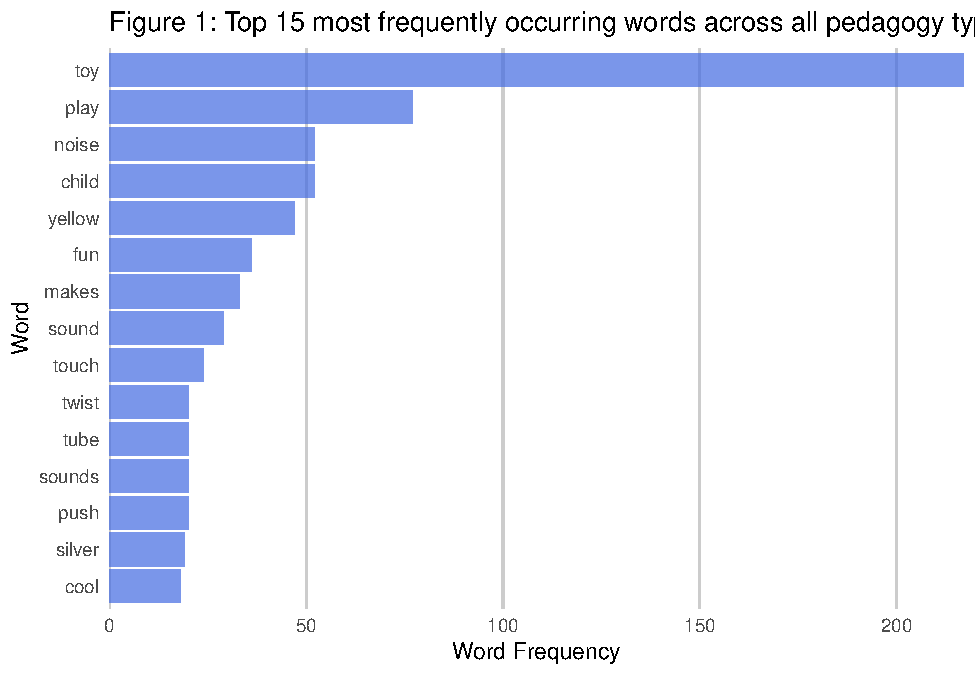
\includegraphics{capstone640_files/figure-latex/initial plots-1.pdf}

\hypertarget{wordcloud-for-overall-sentiment}{%
\subsubsection{Wordcloud for overall sentiment}\label{wordcloud-for-overall-sentiment}}

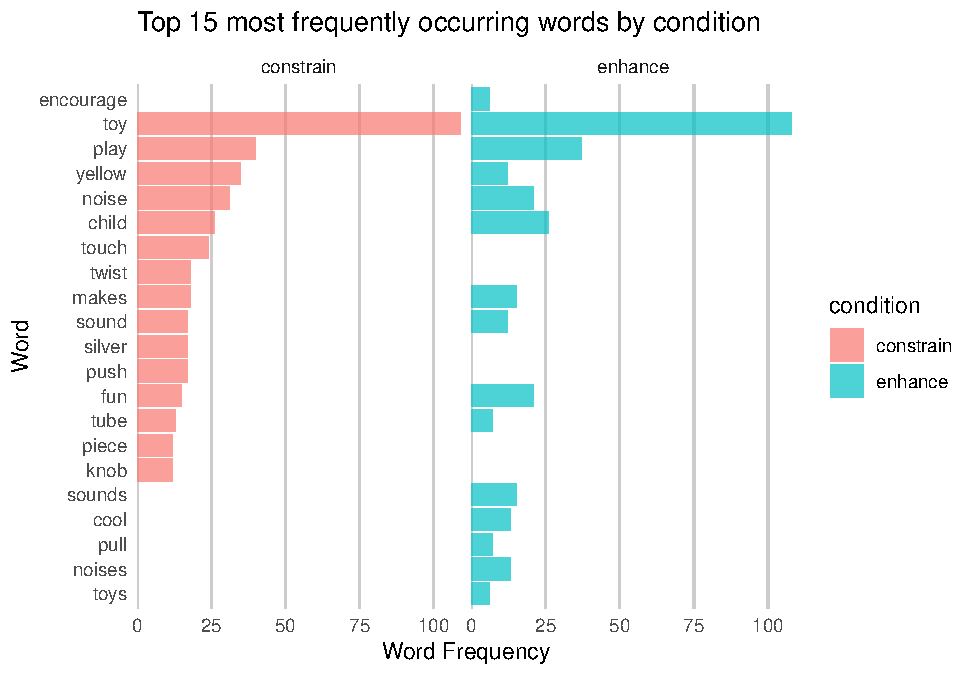
\includegraphics{capstone640_files/figure-latex/unnamed-chunk-1-1.pdf}

\hypertarget{wordcloud-for-positive-sentiment}{%
\subsubsection{wordcloud for positive sentiment}\label{wordcloud-for-positive-sentiment}}

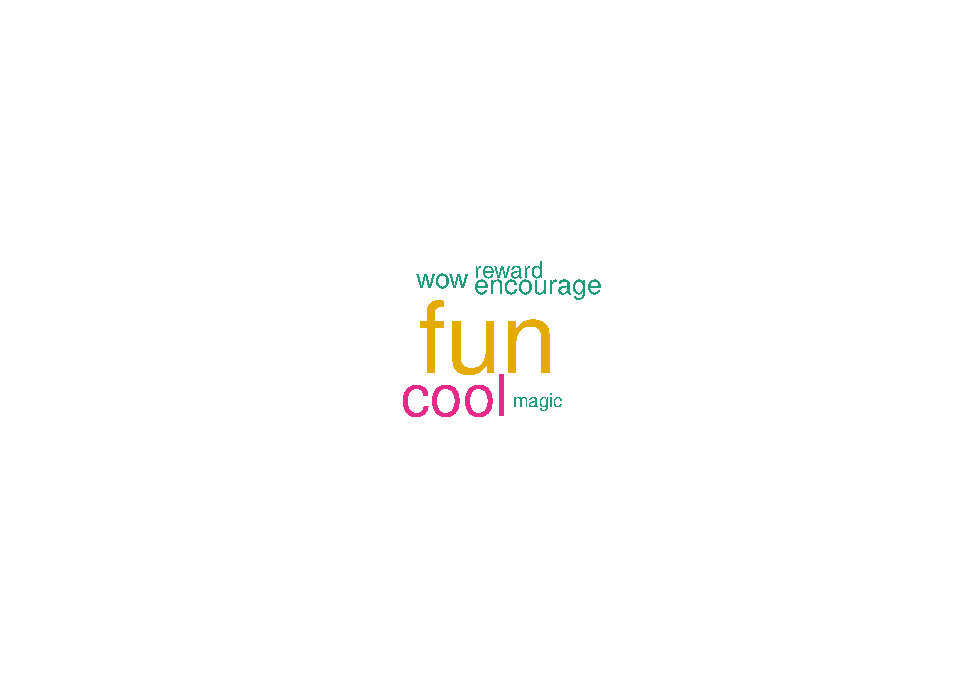
\includegraphics{capstone640_files/figure-latex/unnamed-chunk-2-1.pdf}

\hypertarget{wordcloud-for-negative-sentiment}{%
\subsubsection{Wordcloud for negative sentiment}\label{wordcloud-for-negative-sentiment}}

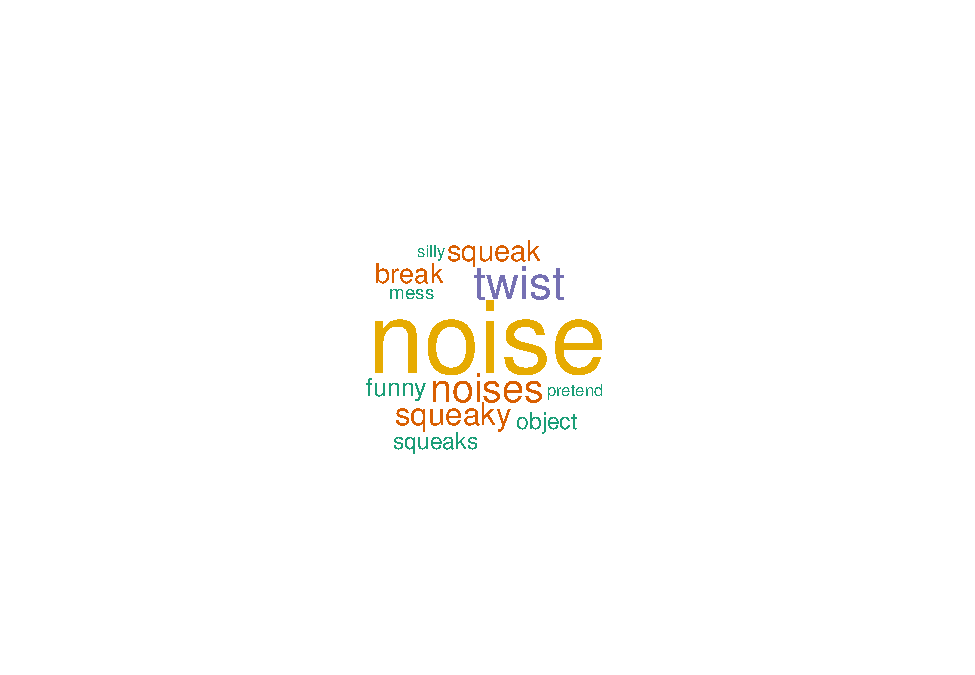
\includegraphics{capstone640_files/figure-latex/unnamed-chunk-3-1.pdf}

\hypertarget{sentiment-radar-chart}{%
\subsubsection{Sentiment Radar Chart}\label{sentiment-radar-chart}}

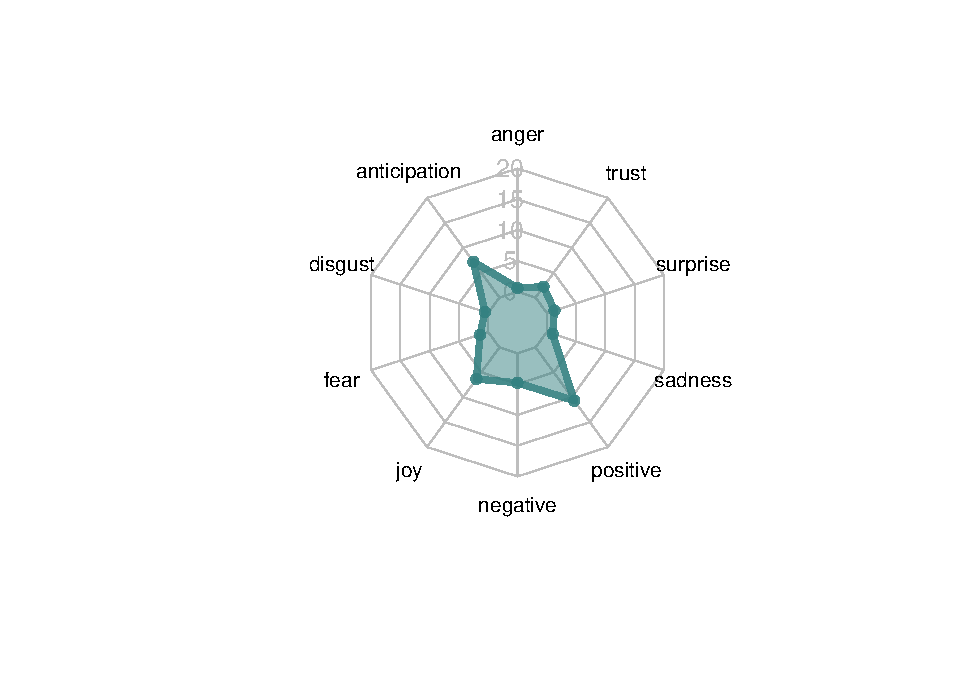
\includegraphics{capstone640_files/figure-latex/unnamed-chunk-4-1.pdf} 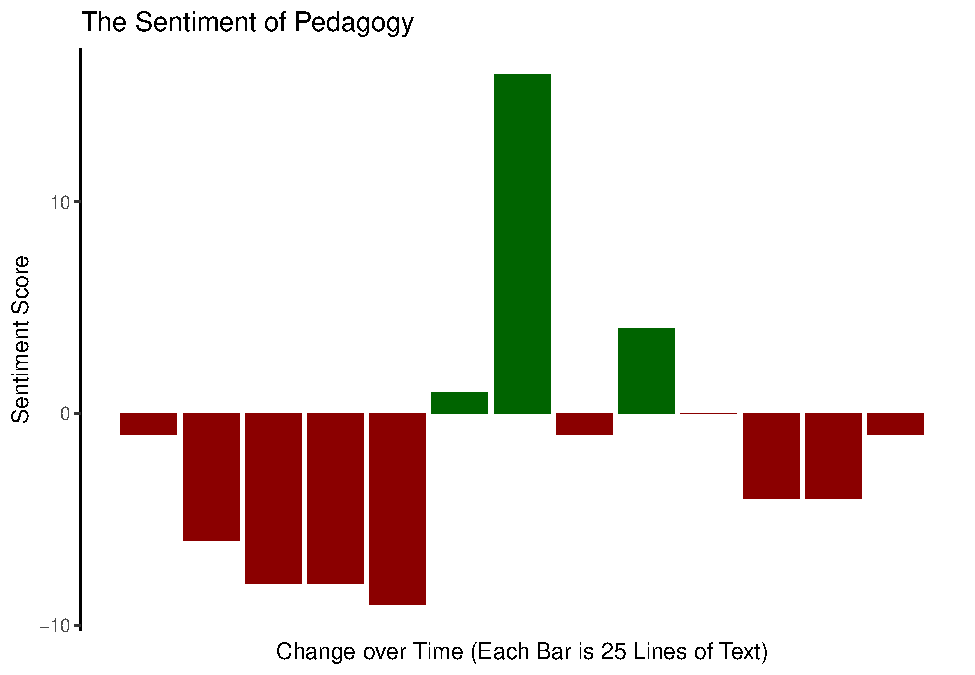
\includegraphics{capstone640_files/figure-latex/unnamed-chunk-4-2.pdf}

\begin{verbatim}
## 
##  ADJ  ADV  AUX INTJ NOUN  NUM PART PRON VERB    X 
##  157   46    1   62  956    1    5    4  349   26
\end{verbatim}

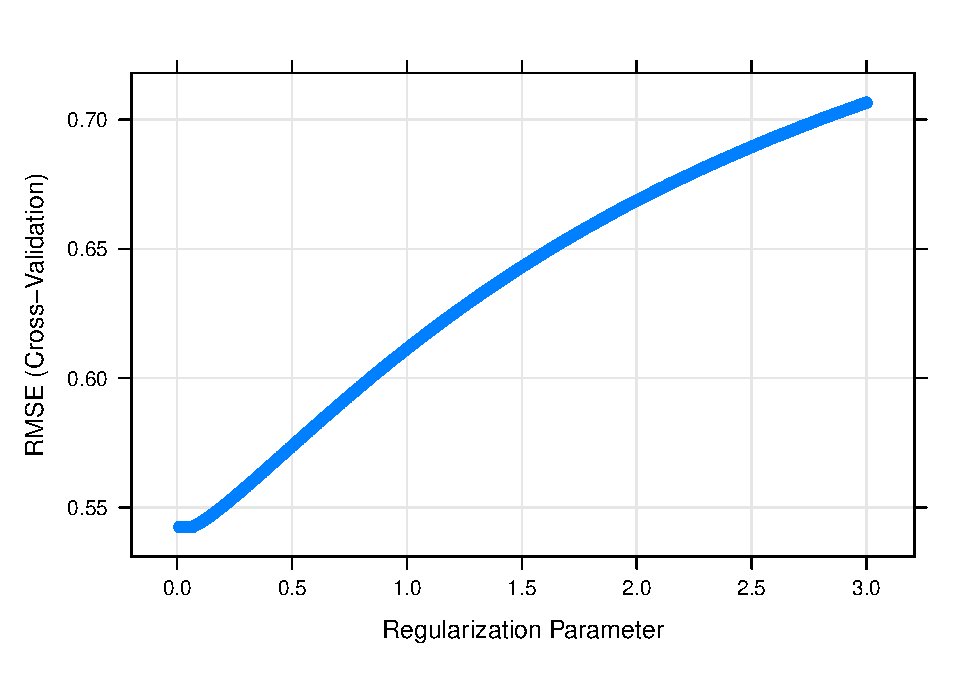
\includegraphics{capstone640_files/figure-latex/unnamed-chunk-5-1.pdf}

\hypertarget{data-analysis-logistic-regression-in-progress}{%
\subsection{Data analysis: Logistic regression (in progress)}\label{data-analysis-logistic-regression-in-progress}}

\hypertarget{results-in-progress}{%
\section{Results (in progress)}\label{results-in-progress}}

\hypertarget{discussion-in-progress}{%
\section{Discussion (in progress)}\label{discussion-in-progress}}

\newpage

\hypertarget{references}{%
\section{References}\label{references}}

We used packages from R {[}Version 4.1.1; R Core Team (2021){]} and the R-package \emph{papaja} {[}Version 0.1.0.9997; Aust and Barth (2020){]} for all our analyses.

\begingroup
\setlength{\parindent}{-0.5in}
\setlength{\leftskip}{0.5in}

\hypertarget{refs}{}
\begin{CSLReferences}{1}{0}
\leavevmode\vadjust pre{\hypertarget{ref-R-papaja}{}}%
Aust, F., \& Barth, M. (2020). \emph{{papaja}: {Create} {APA} manuscripts with {R Markdown}}. Retrieved from \url{https://github.com/crsh/papaja}

\leavevmode\vadjust pre{\hypertarget{ref-R-base}{}}%
R Core Team. (2021). \emph{R: A language and environment for statistical computing}. Vienna, Austria: R Foundation for Statistical Computing. Retrieved from \url{https://www.R-project.org/}

\end{CSLReferences}

\endgroup


\end{document}
